\chapter{写给大家看的 CuTe 教程：TMA Copy}

\begin{center}\small 作者：竹熙佳处（知乎专栏「CuTe 教程」）\quad 原文：\url{https://zhuanlan.zhihu.com/p/2003198909405763007}\end{center}

\section{动机}

Nvidia 在 Hopper 架构[1]之中引入了非常多的新特性，其中 \textbf{Tensor Memory Accelerator (TMA)} 作为新的 load \& store 单元是一个有着深远影响的改动：硬件层面上，从 Hopper 到 Blackwell 架构都延续并强化了 TMA 设计，甚至在 RTX5080 (sm120，blackwell) 这类非计算卡上都被保留了，可以预期后续多代 GPU 都会延续这个设计；软件层面上，其引入正式强化了 \textbf{warp-specialized (WS)} 编程范式的效率，目前正成为 NV tensor core kernel 的标准写法（如 CUTLASS 3.x），足以说明其重要性。

我们观察 NV GPU 架构的演进趋势，可以看到的是越来越高的 IO 带宽以及越来越强的 tensor core。一方面，IO 带宽的增加需要让每个 SM 保持足够大量的数据在 load 过程中（i.e. more bytes in flight，littles-law[2]）才能达到理论带宽上限；另一方面，tensor core 的算力要发挥出来，也需要时刻保持 tensor core 所需的数据是 ready 的状态，否则计算单元将处于 stall 状态，kernel 的计算效率不可能高。

这对于传统的 load 指令提出了挑战。即使我们使用最大字长的指令\textbf{ LDG.128}，一个 warp 单次 load 的数据也只能达到 16Bytes * 32 = 512 Bytes。由于一个 SM 驻留的 warp 数量（Occupancy）是有上限的，因此其能达到的 bytes in flight 往往不足以填满显存带宽。

这时候可以考虑连续多次发射 load 指令（即，ILP），来让更多数据处于 flight 状态。然而增加到一定程度后，就引入了新问题：每条 \verb|LDG| 指令需要消耗寄存器来暂存数据，而寄存器资源的稀缺性反过来限制了 SM 中驻留的 warp 数量，导致 bytes in flight 再次受限，此消彼长，带宽利用率依旧上不去。更不用说在 GEMM / Attention 场景下，寄存器资源多被用于存储 Tensor Core 的累加结果，本就捉襟见肘。

另一个痛点是，频繁的 load 指令发射占用了 warp scheduler 的发射带宽，且 load 伴随的地址计算也会加重 ALU 的负担，进一步挤压了能达到的 load 带宽。

于是，机智的 NV 工程师提出了新的解法：

\begin{itemize}
  \item 既然多条指令 load 效率低，那么把单条指令能 load 的数据量增大；
  \item 寄存器资源受限，那么 Bypass Register，直接将数据 load 到空间相对更充裕的 shared memory 中；
  \item 地址计算消耗 ALU，那让地址计算在专用硬件上完成。
\end{itemize}

因此，在 Hopper 架构中，TMA 应运而生：

\begin{itemize}
  \item 其可以做到一条 \textbf{cp.async.bulk.tensor }指令 load 一整块数据到 shared memory。TMA 作为一个专有硬件单元，可以自行完成地址计算，甚至自带越界(OOB) 处理 ，相当贴心。
  \item 同时，TMA 作为 Global Memory 到 Shared Memory 之间的传输单元，是完全异步执行的。即，其具体什么时候完成 Copy 需要通过 \textbf{mbarrier} 来同步，在使用 Shared Memory 的数据前必须 wait barrier 以确保数据正确性。
  \item 为了针对性优化 Tensor Core 计算中常用的 Tile data 加载，TMA 被设计为支持多维数据访问，即，\textbf{对于 TMA 来说内存空间不再是一个连续的 1 维地址空间，而是一个多维 box 空间，支持 1D\textasciitilde{}5D 的数据访问}。
\end{itemize}

有了 TMA，我们就可以达到极高的 load 效率，在 Memory-bound kernel 中尽可能跑满带宽，在 Compute-bound kernel 中通过更好的 Overlap 让 Tensor Core 零等待，尽可能达到算力上限。在硬件上，TMA 作为一个独立硬件单元，物理位置紧邻 Shared Memory，每个 SM 标配一个 TMA 单元，如 Fig.1 所示。

\begin{figure}[htbp]\centering

\includegraphics[width=0.9\textwidth]{figures/zhuxi-05-tma-copy/fig-01.jpg}
\caption{Figure.1 Hopper SM 架构图；每个 SM 均配有一个 TMA，其位置位于 Shared mem 之上}
\end{figure}

\section{用法}

那么如何才能使用 TMA 呢？首先我们以 2D load 为例，高度概括地总结一下其基本流程。

\textbf{Host 端：构造 TMA Descriptor }

在 Host 端完成 TMA Copy Descriptor 的构造，并将其作为 Kernel 参数传入。语义上，它包含：

\begin{itemize}
  \item \textbf{Global Memory 信息}： Base Pointer、整体 Layout (Shape \& Stride)；
  \item \textbf{Box 信息}： 每次 Copy 搬运的数据块（Box）的 Shape \& Stride；
  \item \textbf{控制信息}： Swizzle 模式、OOB（越界）处理模式、L2 Cache 策略等。
\end{itemize}

这个 Descriptor 本质上是底层硬件使用的一段连续的 128 Bytes 数据，具体的字段对用户不透明，在不同 arch 以及驱动版本都有着不同的含义。

\textbf{Kernel 端：发起 Copy 指令}

在 Kernel 内通过调用 \textbf{ cp.async.bulk }指令发起 Copy，同时提供：

\begin{itemize}
  \item \textbf{Descriptor}： 即 Host 端传进来的对象；
  \item \textbf{Mbarrier}： 用于控制是否 copy 完成的对象；
  \item \textbf{Dst Pointer}： Shared Memory 的目标地址；
  \item \textbf{Coordinates}： 要访问的数据块在 Global Tensor 中的逻辑坐标，例如 2D，就需要 2 个数值 crd0 \& crd1 来代表坐标，以 Descriptor 中 的 Base Pointer 为起始。
\end{itemize}

然后等待 mbarrier 到达预期状态，Copy 结束，Shared Memory 数据准备就绪。这个过程我们可以描述为 Fig.2。

\begin{figure}[htbp]\centering

\includegraphics[width=0.9\textwidth]{figures/zhuxi-05-tma-copy/fig-02.jpg}
\caption{Figure 2. 2D TMA copy 过程示意图；在 Host 端完成 TMA Descriptor 的构造，在 Kernel 中完成 TMA Copy，每次 Copy 完成一个 Box 大小的数据搬运，依靠 Mbarrier 来标记 Copy 完成}
\end{figure}

以上过程，Old-school 选手可能会使用 cuda 提供的 API，来指定对应参数后创建一个 CUtensorMap 结构体作为 descriptor。然后用 inline ptx 的方式调用 \textbf{cp.async.bulk.tensor} 指令，以及相关的 \textbf{mbarrier} 指令来等待 barrier 完成。如果不想深度依赖 CuTe layout 体系，也可以使用 CuTe 已有的封装好的 ptx 函数，deepgemm 就是借用的这种方式。

\begin{lstlisting}[language=C++]
CUTE_HOST_DEVICE static void
  copy(void const* desc_ptr, uint64_t* mbar_ptr, uint64_t cache_hint,
       void      * smem_ptr,
       int32_t const& crd0, int32_t const& crd1) {
    uint64_t gmem_int_desc = reinterpret_cast<uint64_t>(desc_ptr);
    uint32_t smem_int_mbar = cast_smem_ptr_to_uint(mbar_ptr);
    uint32_t smem_int_ptr  = cast_smem_ptr_to_uint(smem_ptr);
    cutlass::arch::synclog_emit_tma_load(__LINE__, gmem_int_desc, smem_int_mbar, smem_int_ptr);
    asm volatile (
      "cp.async.bulk.tensor.2d.shared::cluster.global.mbarrier::complete_tx::bytes.L2::cache_hint"
      " [%0], [%1, {%3, %4}], [%2], %5;"
      :
      : "r"(smem_int_ptr), "l"(gmem_int_desc), "r"(smem_int_mbar),
        "r"(crd0), "r"(crd1), "l"(cache_hint)
      : "memory");
  }
\end{lstlisting}

更简单的，CuTe 已经提供了足够简洁的上层函数如 make\_tma\_copy / get\_tma\_tensor / copy 函数来完成上述步骤，我们遵循 CuTe 的使用方法即可，在此我们引用 coflex 的经典文章[3]中的代码段（原代码竟然还有 bug，不过瑕不掩瑜，大体流程是正确的）来展示其用法。

TMA copy descriptor 的构造如下代码：

\begin{lstlisting}[language=C++]
template <typename T, int CTA_M, int CTA_N>
void host_fn(T* data, int M, int N) {
  using namespace cute;
 
  // 1. Create the GMEM tensor
  auto gmem_layout = make_layout(make_shape(M, N), LayoutRight{});
  auto gmem_tensor = make_tensor(make_gmem_ptr(data), gmem_layout);
 
  // 2. Create the SMEM layout (Atom layout for TMA)
  auto smem_layout = make_layout(make_shape(CTA_M, CTA_N), LayoutRight{});
 
  // 3. Create the TMA object (contains the Tensor Map)
  auto tma_load = make_tma_copy(SM90_TMA_LOAD{}, gmem_tensor, smem_layout);
 
  // 4. Invoke the kernel
  tma_load_kernel<T, CTA_M, CTA_N, decltype(tma_load),
                                           decltype(gmem_layout),
                                           decltype(smem_layout)><<<dim3{M / CTA_M, N / CTA_N, 1}, 1>>>(data, tma_load, gmem_layout, smem_layout);
}
\end{lstlisting}

copy 执行代码如下：

\begin{lstlisting}[language=C++]
template <typename T, int CTA_M, int CTA_N, class TmaLoad, class GmemLayout,
          class SmemLayout>
__global__ void tma_load_kernel(T* g_out, const T* g_in,
                                __grid_constant__ const TmaLoad tma_load,
                                GmemLayout gmem_layout,
                                SmemLayout smem_layout) {
  using namespace cute;
  constexpr int tma_transaction_bytes = CTA_M * CTA_N * sizeof(T);

  __shared__ T smem_data[CTA_M * CTA_N];
  __shared__ uint64_t tma_load_mbar;

  // Construct SMEM & GMEM tensor
  Tensor smem_tensor = make_tensor(make_smem_ptr(smem_data), smem_layout);
  Tensor gmem_tensor = make_tensor(make_gmem_ptr(g_in), gmem_layout);

  if (threadIdx.x == 0) {
    auto gmem_tensor_coord = tma_load.get_tma_tensor(shape(gmem_tensor));

    auto gmem_tensor_coord_cta = local_tile(
        gmem_tensor_coord, Tile<Int<CTA_M>, Int<CTA_N>>{},
        make_coord(blockIdx.x, blockIdx.y));

    initialize_barrier(tma_load_mbar, /* arrival count */ 1);
    set_barrier_transaction_bytes(tma_load_mbar, tma_transaction_bytes);

    auto tma_load_per_cta = tma_load.get_slice(0);
    copy(tma_load.with(tma_load_mbar),
         tma_load_per_cta.partition_S(gmem_tensor_coord_cta),
         tma_load_per_cta.partition_D(smem_tensor));
  }
  __syncthreads();
  wait_barrier(tma_load_mbar, /* phase */ 0);
  // after this line, the TMA load is finished
}
\end{lstlisting}

如果只是想了解如何使用，那么上面的例子抄下来改一改就可以了，这其实也是对 CuTe 熟悉之后的好处：能够对照 cutlass 快速开发算子，尽管对硬件细节没有那么了解。但是本专栏的读者朋友，大概不会满足于如此粗浅的了解，接下来我们更深入的了解一下 CuTe 中关于 TMA 的细节。

\section{CuTe 中的坐标表示: arithTuple}

首先，我们思考 TMA copy 和普通的 SIMT copy 有什么不同：我们可以注意到，\textbf{SIMT copy 本质上是每个 thread 每条指令消耗一个 1d offset，而 TMA copy 则是消耗一个起始坐标}。我们可以看到上述代码中的 \textbf{get\_tma\_tensor} 函数就是构建了这样一个 gmem\_tensor\_coord，其在 CuTe 中定义如下：

\begin{lstlisting}[language=C++]
auto get_tma_tensor(GShape const& g_shape) const {
    static_assert(is_congruent<decltype(g_shape), decltype(aux_params_.g_stride_)>::value);
    return make_coord_tensor(make_layout(g_shape, aux_params_.g_stride_));
  }
\end{lstlisting}

为什么这里不是一个普通的 make\_tensor 就可以了呢？因为 CuTe Layout 的主要功能是用来把坐标转换成 1d offset，而在 TMA 场景下，我们需要保留原始的 ND 坐标语义，不需要转换成 1d offset，因此常规的 Layout 语义在这里是不匹配的。

为此，CuTe 只能打个补丁，引入了一个新的概念来表示纯粹的坐标语义，此即 \textbf{arithTuple}。 我们先结合一个例子来理解 arithTuple 如何表示坐标：

\begin{lstlisting}[language=C++]
Tensor a = make_tensor(make_inttuple_iter(0,0),
                       make_shape (     4,      5),
                       make_stride(E<0>{}, E<1>{}));
print_tensor(a);
/*
ArithTuple(0,0) o (4,5):(_1@0,_1@1):
  (0,0)  (0,1)  (0,2)  (0,3)  (0,4)
  (1,0)  (1,1)  (1,2)  (1,3)  (1,4)
  (2,0)  (2,1)  (2,2)  (2,3)  (2,4)
  (3,0)  (3,1)  (3,2)  (3,3)  (3,4)
*/
\end{lstlisting}

可以看到，我们仍然用 make\_tensor 创建了 tensor，只不过这个 tensor 比较特殊，其 “base\_ptr” 不再指向一个内存地址，而是一个 tuple，用来表示起始坐标 (0, 0)。 然后对于其 “layout” 部分，我们也用 shape \& stride 表达：其中 shape 的表示是平凡的；stride 则需要注意——由于需要表示 2D 的位置变化，我们需要指定一个“2D stride”。

就这个例子而言，我们希望在每一列上，逐行增加第一个维度的坐标，因此第一个维度 stride 设为 (1, 0)；同理，我们希望在每一行上逐列增加第二个维度的坐标，因此第二个维度 stride 设为 (0, 1)。 语义上，我们可以理解成 make\_stride((1, 0), (0, 1))。 但为了避免歧义并简化表达，CuTe 将 (1, 0) 和 (0, 1) 这类基础步长定义为\textbf{ Basis Element，表示为 E$<$0$>$\{\} 和 E$<$1$>$\{\}}。这其实和普通 Layout 中用 Int$<$1$>$\{\} 作为 stride 是类似的。

具体的，这个 E$<$0$>$\{\} 代表的是“第 0 个位置为 1，其他位置为 0 ” 的 tuple；E$<$1$>$\{\} 代表的则是“ 第 1 个位置为 1，其他位置为 0”。从其 print 结果来看，(\_1@0, \_1@1) 其实就是在表达这样一个语义：\textbf{\_1@0 代表第 0 位置的 stride 为 1（@0 代表 at 0 维度），\_1@1 代表第 1 位置的 stride 为 1}。 E 可以乘以一个整数表示 stride 的扩大，如我们把例子中的 stride 改为 (5 * E$<$0$>$\{\}, 2 * E$<$1$>$\{\})，其打印结果如下：

\begin{lstlisting}[language=C++]
Tensor a = make_tensor(make_inttuple_iter(0,0),
                       make_shape (     4,      5),
                       make_stride(5 * E<0>{}, 2 * E<1>{}));
print_tensor(a);
/*
ArithTuple(0,0) o (4,5):(5@0,2@1):
  (0,0)  (0,2)  (0,4)  (0,6)  (0,8)
  (5,0)  (5,2)  (5,4)  (5,6)  (5,8)
  (10,0)  (10,2)  (10,4)  (10,6)  (10,8)
  (15,0)  (15,2)  (15,4)  (15,6)  (15,8)
*/
\end{lstlisting}

有了基于 arithTuple 的坐标表示，我们就可以着手构建 TMA copy 相关的函数了。我们知道普通的 CuTe Tensor 是由一个 base\_ptr + layout 构成的，那么将 base\_ptr 替换为一个 base 坐标，Layout 也替换为对坐标的 Shape \& Stride 描述，这就构成了 TMA Tensor。

那么这种特殊的 Tensor，是否仍然适用于我们在普通 Tensor 上定义的各种函数，如 Partition \& Tile？其 Layout 是否也能做到通过 Inverse \& Compose \& Product \& Divide [4][5]灵活变换呢？

答案是肯定的。事实上我们从前面的代码中也可以看到，对 gmem\_tensor\_coord\_cta 仍然可以用 \textbf{local\_tile} 以及 \textbf{partition\_S} 函数来进行数据划分。这在大体上保证了不同架构（SIMT vs TMA）的 Kernel 在写法和逻辑上的统一。

另外一个需要注意的点，是 TMA Box 的起始坐标，不一定需要是和 Box Size 对齐的。比如 Box Size 是 (16, 64)，起点可以是 (0, 8) 这样的位置，只要满足起点对应到 global mem 上的物理地址是 16 Bytes 对齐即可。这也是处理 variable-len Attention 或是 Group GEMM 下的常用特性，通过坐标的 domain\_offset 函数即可完成起始位置的偏移。

顺带一提，在 CuTe 中，arithTuple 除了用来表示 TMA 坐标，也可以用来构建 Identity Tensor，进而用于处理 Tiled Copy 的边界判定或是 Attention 中 Mask 的逻辑，也是非常实用的特性。

\section{MBarrier}

TMA 是一个异步 copy 单元，其 copy 的完成是无法预测的，需要显式 wait barrier 达到某个特定状态，才能认为 copy 得到的数据可用。那么这个 barrier 具体是如何发挥作用的呢？对应的 CuTe 函数是如何修改 / 检查 barrier 的状态呢？

实际上，我们可以把 barrier 认为就是一个 \verb|uint64_t| 的变量，通常声明在 shared memory，其特殊之处在于 64 个 bit 位都被赋予了特定语义。例如，我们把相关代码抽出来看，\verb|tma_load_mbar| 就是一个 barrier。

\begin{lstlisting}[language=C++]
constexpr int tma_transaction_bytes = CTA_M * CTA_N * sizeof(T);
  __shared__ uint64_t tma_load_mbar;
  if (threadIdx.x == 0) {
    initialize_barrier(tma_load_mbar, /* arrival count */ 1);
 
    set_barrier_transaction_bytes(tma_load_mbar, tma_transaction_bytes);
 
    copy(tma_load.with(tma_load_mbar),
         tma_load_per_cta.partition_S(gmem_tensor_coord_cta),
         tma_load_per_cta.partition_D(smem_tensor));
  }
  __syncthreads();
  wait_barrier(tma_load_mbar, /* phase */ 0);
\end{lstlisting}

那么这 64-bit 都包含哪些信息呢？在 NV open AI day 的技术分享中，其展示了 barrier 各字段语义如 Fig.3：

\begin{figure}[htbp]\centering

\includegraphics[width=0.9\textwidth]{figures/zhuxi-05-tma-copy/fig-03.jpg}
\caption{Figure 3. Barrier 包含的语义表示。包含一个 1bit 翻转用的 Phase 段，预期的 arrive count 以及 transaction bytes，以及实际被执行的 arrive count 以及 transaction bytes。实际 transaction bytes 则只能通过 tma 指令来改变。}
\end{figure}

具体来说，语义上，barrier 这些字段中包含我们可以指定的两个初始量：

\begin{itemize}
  \item \textbf{Expect arrv\_cnt}：代表期望有多少个 producer 线程到达（arrive），通过 initialize\_barrier 函数设置。
  \item \textbf{Expect trans\_bytes}：代表期望本次传输需要完成多少 bytes，通过 set\_barrier\_transaction\_bytes 设置。
\end{itemize}

以及随着 copy 的进行，我们可以动态改变的量：

\begin{itemize}
  \item \textbf{Actual arrv\_cnt}：代表\textbf{当前已到达的次数}。代码中 lane 0 发起 copy 前会进行 arrive 操作，该数值 +1。
  \item \textbf{Actual trans\_bytes} (只有 TMA 硬件能改)：代表实际传输了多少 bytes，tma 每完成一部分 bytes 的 copy，就会更新这个字段。
  \item \textbf{phase}：1 bit，初始化为 0，且是一个可以在 0-$>$1 / 1-$>$0 之间翻转的状态量。所谓 \verb|wait_barrier| 就是在等待其产生变化。
\end{itemize}

TMA 在传输完成后，barrier 状态若同时满足：\textbf{Actual arrv\_cnt == Expect arrv\_cnt} 且 \textbf{Actual trans\_bytes == Expect trans\_bytes}，那么这个 phase 位会发生翻转。

例如，初始 phase 为 0，TMA copy 完成后，phase 发生 0 -$>$ 1 的翻转，那么 wait\_barrier(barrier, 0) 这个阻塞就被解除了，这条指令之后的指令（如 mma）就可以开始执行了。

值得注意的是，如果我们 wait\_barrier(barrier, 1)，那么其在 phase 为 0 时，会直接解除阻塞（因为 0 != 1），只有等到 phase 为 1 时才开始阻塞，并且等待 phase 1 -$>$ 0 的翻转发生后，再解除阻塞。

更细节的 barrier 各字段的精准定义，我们推荐 @reed\footnote{\url{https://www.zhihu.com/people/2600b0313c76a175aa9e09a235382b79}}  的这篇文章：cute 之 Hopper MBarrier\footnote{\url{https://zhuanlan.zhihu.com/p/1962636004235153810}}
值得一提的是，CuTe 中对于 barrier 的使用，通常会被封装到pipeline 的结构体 [6]中，来提供在 multi-stage 场景下的 barrier 状态的管理，只不过在没有文档的情况下，对这个结构体的理解又是非常繁重的心智负担，我们后续再单独出文章进行总结。当然，即使不使用 pipeline，只要理清楚 barrier 的状态变化，我们在 multi-stage 场景下在依旧能用好 barrier，deepgemm 就是一个很好的例子，reed 的 hpc-ops 库[7]也都是这样使用的。

\section{make\_tma\_copy 梳理}

了解完 TMA copy 在 kernel 中如何发起后，我们再回头来看看 TMA 在 host 端的 copy descriptor 是如何构建出来的。 然而在代码层面，我们可以看到核心函数 make\_tma\_copy() 调用一次就完成了，但是其底层代码远比我们想象的要复杂得多。甚至可以将其当作一个微型优化器来理解。

其输入：

\begin{itemize}
  \item copy\_atom
  \item global tensor
  \item shared layout
\end{itemize}

输出一个\textbf{带有最优 TMA descriptor 的 TiledCopy 对象}。

那么这个“最优” 是怎么理解的呢？这里我们需要了解一下 TMA 作为一个硬件单元的特点：

\begin{itemize}
  \item \textbf{维度限制}： 支持 1D\textasciitilde{}5D 的 Box Copy，高于 5D 会报错。
  \item \textbf{Box 大小限制}： 单次 TMA Box 的每个维度元素个数受硬件指令字段限制（8-bit），必须小于等于 256。
  \item \textbf{效率要求}： 在 copy 相同 bytes 的数据时，一次 copy 大块数据比多次 copy 小份数据发射指令更少，因此 copy 效率更高。
\end{itemize}

而我们在使用 CuTe 时，有时会无法避免地写出来非常高维的 Tensor，例如在描述 attention 中 QKV tensor 时，(batch, seqlen, num\_head, head\_dim) 就已经占据了 4 个维度了，再加上我们需要叠加 Swizzle 引入的 shm atom 切分，这就 6 个维度了，完全不够用；类似的情况还有 conv、group gemm 算子等等。

既然硬件不支持 $>$5D 的 Box，那只有在代码层面来对高维数据进行合并；而且考虑到发起的 copy 越少越好，这个合并应该是一个贪心的过程，且在合并的过程中也要检查不能超出硬件对 Box Size 的 256 限制。其具体的逻辑涉及到非常多 CuTe 的代数变换以及多个辅助函数，我们总结其主要函数的调用逻辑为如下伪代码：

\begin{lstlisting}
#输入： 
# copy_atom: SM90_TMA_LOAD / SM90_TMA_LOAD_MULTICAST / SM90_TMA_STORE;
# global tensor，
# shared layout，
# 输出：
# 带有合并维度 TMA descriptor 的 tiled copy 对象
def make_tma_copy(copy_atom, gtensor, slayout, ...):
    # 1. 去除 swizzle 逻辑，只取 shape
    smem_layout_pure = get_nonswizzle_portion(slayout)
    
    # 2. 编译期合并维度 & 构建 TMA descriptor & 检查 256 限制
    def make_tma_copy_atom(gtensor, smem_layout_pure):
        
        # 2.1 compile-time 合并维度: eg. ((_8,_16),(_64,_2)) -> ((_64,_128),_2)
        tma_gbasis = construct_tma_gbasis(gtensor, smem_layout_pure):
            # 尝试将 shm layout 映射回 global layout，方便下一步合并连续的维度
            tile_gstride = gtensor.compose(right_inverse(smem_layout_pure)).layout()
            
            # 按规则合并维度，并检查合并后的维度 <= 256
            tma_gstride = coalesce_256(tile_gstride)
            
            # 返回合并后的维度信息
            return tma_gstride 

        # 2.2 按照合并好的维度构建 TMA descriptor & 必要时将超过 5d 的维度合并成 5d
        tma_desc = make_tma_copy_desc(gtensor, tma_gbasis):
            
            # C. run-time 计算超过 5d 维度的 Stride 最大公约数 (GCD)，进而将其压缩成一个维度
            fill_tma_gmem_shape_stride(gtensor, tma_gbasis, output=tma_desc)
            
            # D. 可选：根据 multicast 属性切分 tma box size
            if is_multicast:
                smem_box_shape = ceil_div(smem_box_shape, multicast)
            
            # E. 调用 CUDA 驱动 API，生成 TMA descriptor 
            cuTensorMapEncodeTiled(tma_desc, ...)
            
            return tma_desc

        # 3. 返回封装好的 tiled copy 对象
        return TiledCopy(tma_desc, layout_TV)
\end{lstlisting}

初读 CuTe 中的这段代码，笔者也感到非常困惑，我们用 TMA 只不过想完成一个 Tile 数据的 copy，至于引入这么多复杂逻辑吗？但是经过思考我们发现，这些逻辑其实就是为了应对复杂 Layout 场景下（如引入 Swizzle），自动生成我们上述提到的 “最优” copy 方案。

举个例子，我们在对一个简单的 (128, 128) bf16 的 Tile 进行 swizzle 的切分后，其 shape 变为了 ((8, 16), (64, 2))。按照最朴素的想法，应该设置 Box Size 为 (8, 64) 然后发起 16x2 次 copy。但是实际上经过 make\_tma\_copy 的优化，你会发现其打包成了\textbf{ (128, 64)}，大大减少了指令发射数量。

为什么可以这样合并呢？因为 (8, 64) 的 atom layout 按照 col-major 排列，那么在 M 维度上的 16 个 atom 实际上在内存上是连续的，\textbf{construct\_tma\_gbasis() }会贪心地将其合并起来。

那么，为什么不在 N 维度上继续贪心扩展到 128 呢？这是因为 \textbf{Swizzle Mode }决定了 TMA Box 在连续维度的最大物理宽度。对于 bf16 (2 Bytes) 来说，128 Bytes / 2 = 64 个元素。

\begin{figure}[htbp]\centering
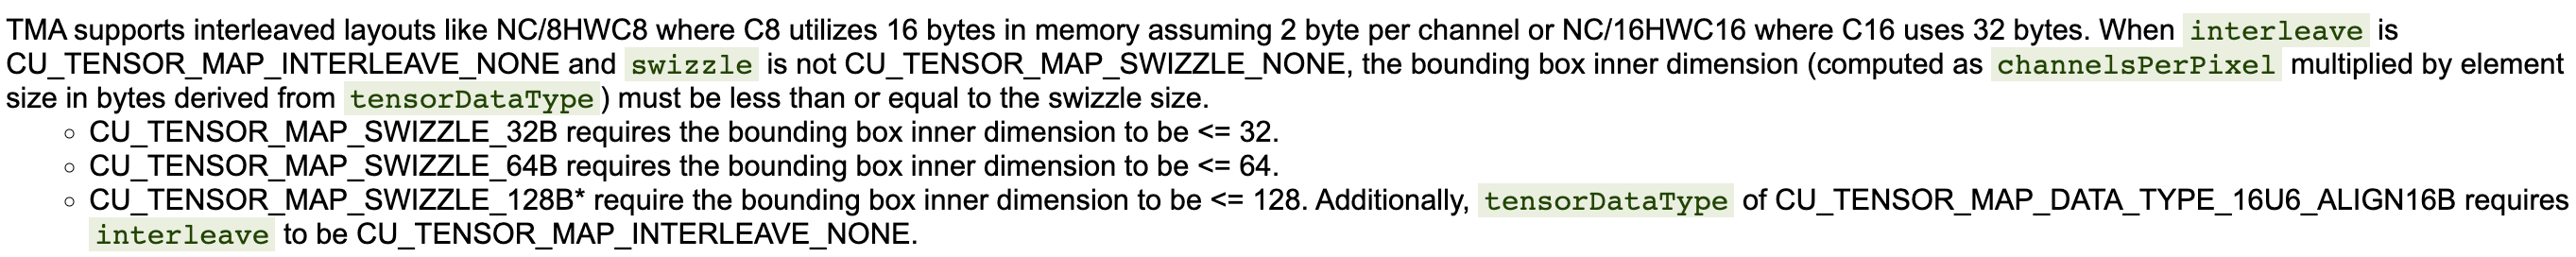
\includegraphics[width=0.9\textwidth]{figures/zhuxi-05-tma-copy/fig-04.png}
\end{figure}

这个限制会体现在 SMEM Layout 上，并由此传递给了 make\_tma\_copy() 函数，最终生成了符合硬件约束的最优 Box Size。

TMA 除了可以做到简单的数据 copy，还可以做到一次 load 数据写出到多个 SM 上的 shared mem 上（要求这些 SM 在同一个 cluster 上）。例如，我们在 gemm kernel 这类存在数据复用的场景，可以做到一个 TileA 广播给 SM0 和 SM1 使用，这样对于 SM0 和 SM1 来说，只需要各自读取 1/2 TileA 的数据并 multicast 给对方，就可以正常完成后续的 gemm 操作了，能大大减少 load 的数据量，是一个非常实用的功能。

在 CuTe 中，其做法就是将 TileA 的上半部分交给 SM0 copy，TileA 的下半部分交给 SM1 copy。这时候虽然 SM0 和 SM1 的 tma 各自只 load 了 1/2 TileA 数据，但是每个 SM 都收到了 TileA 的数据量，所以我们设置 transaction bytes 也仍然是完整 TileA 的量，原则就是每个 sm 并不关心自己的 TMA 发了多少数据的 copy，只管自己接收到了多少数据。

读者可能有疑问，为什么不直接拆分为左右各一条 tma copy 然后 multicast？我猜测这里是为了通用性考虑，因为 tile size 可能是 64 的奇数倍，例如 192，这时候如果做左右拆分，会有一条 copy 指令只有一个 SM 在做，另一个 SM 在等待，且不说性能会不如均分（max(2, 1) $>$ mean(2, 1)），可维护性也是个大问题。

我们可以将上述 make\_tma\_copy 描述过程展示如 Fig.4。

\begin{figure}[htbp]\centering

\includegraphics[width=0.9\textwidth]{figures/zhuxi-05-tma-copy/fig-05.jpg}
\caption{Figure 4. make\_tma\_copy() 执行流程。包含贪心合并 TMA 维度，descriptor 的生成，multicast 处理等流程，得到最优的 copy 方案。}
\end{figure}

在上述的介绍中，我们提到 \textbf{fill\_tma\_gmem\_shape\_stride()} 这个函数会对超过 5D 的数据进行压缩，在此我们给读者朋友一个挑战：

尝试思考一下其是如何做这个压缩的（为什么用到 GCD 最大公约数），这个压缩并不完美，其潜在问题是什么。如果读者对这个部分也能思考清楚，可以认为你对 TMA 有了相当清楚的认知，我们在评论区给出答案，也欢迎大家给出自己的看法。

\section{TMA proxy \& fence}

通过 TMA 来 load / store shared mem，和正常 sts 以及 lds 指令访问 shared mem 所走的数据通路（后者走 Load Store Unit, LSU）是不同的，但是其访问的数据又有可能是同一段地址。这时两个访问方式就被称为两个 Proxy：正常走 LSU 的 proxy 被称为 \textbf{Generic Proxy}，TMA 走的 proxy 被称为 \textbf{Async Proxy}。

不同 proxy 访问同一块地址会出现内存可见性的问题，因为硬件之间无法即时同步这个地址的读写状态，因此要加一个 \textbf{fence} 来保障跨 Proxy 的内存可见性。

例如，在 GEMM Kernel 中，通常在计算完成需要输出结果到 Global Memory 时，会先从 Register Copy 到 Shared Mem 中（不管调用的是 stmatrix 还是 sts 指令，其对应的硬件单元都是 LSU），然后再经由 TMA 发起从 Shared Mem 到 Global Mem 的 Copy。这里为了保证 TMA 搬运的数据是 LSU 刚刚写入的最新的数据，必须要在两者之间加一个 TMA Fence，其指向的 ptx 代码如下：

\begin{lstlisting}[language=C++]
// Issue a shared memory fence for async operations
CUTLASS_DEVICE
void fence_view_async_shared() {
#if CUDA_BARRIER_ENABLED
    cutlass::arch::synclog_emit_fence_view_async_shared(__LINE__);
    asm volatile (
        "{\n\t"
        "fence.proxy.async.shared::cta; \n"
        "}"
        ::
        : "memory");
#else
    CUTLASS_NOT_IMPLEMENTED();
#endif
}
\end{lstlisting}

这里值得注意的是，\textbf{fence 和 sync (\_\_syncthreads 或是 named barrier sync) 是两个不同维度的原语}。

\verb|__syncthreads| 仅保证了 Generic Proxy 下的线程同步和内存一致性（即，确保所有线程都已经把数据写进 shared mem），但它\textbf{并不保证}跨 Proxy 的可见性。 因此，如果只做 sync 不做 fence，TMA 单元可能看不到 LSU 刚刚写入的数据；反之，如果只做 Fence 不做 Sync，TMA 发起时可能其他线程还没写完数据。

所以，正确的流程通常是：先 \textbf{sync}（确保数据就绪），再 \textbf{fence}（确保 TMA 可见），最后发起 \textbf{TMA Store}。那么 sync 的时候为什么不把 fence 一起做了呢？因为这个操作只有在涉及跨 Proxy（如 STS 和 TMA 混用）的特定场景下才需要。如果在所有 sync 中都强制加入 fence，在大量不需要跨 Proxy 交互的场景下（例如纯 CUDA Core 计算）会引入不必要的开销，得不偿失。

\section{总结}

本文介绍了从 Hopper 架构开始引入的 \textbf{Tensor Memory Accelerator (TMA)，其出现是为了充分利用 GPU 越来越高的 IO 带宽，确保 IO bound 和 Compute bound kernel 都能达到预期性能。}具体的，其实现了仅需一条指令即可将整块 Tile 搬运至 Shared Memory，从而释放了带宽潜力。

然而，代价是什么？

TMA 的出现深刻改变了 GPU 的编程范式，并引入了一系列新概念，如 descriptor，barrier，proxy 等等，对于一个从 Ampere 架构下切换过来的开发者来说是一个不小的心智负担。

好在我们可以借助 \textbf{CuTe} 来驾驭这一硬件特性。因此，我们在本文中重点介绍了\textbf{ CuTe 坐标体系}，\textbf{MBarrier 的 Phase 翻转机制}，并重点解读了 \textbf{make\_tma\_copy 函数}，其能够针对硬件的维度限制和 Box Size 限制进行贪心的维度合并来最大化带宽，并能够很好的处理 multicast 场景。最后我们讨论了保证 Generic/Async Proxy 内存可见性的 \textbf{fence} 机制，确保写出的 kernel 的数据正确性。

笔者的一个感受就是，CuTe 的核心代码确实难读，但是好处是其经过开源的检验，并有 CUTLASS / Flash Atten 这样可以借鉴的高质量代码库。笔者曾经参与维护过一套手写 PTX 搭建的 TMA + WGMMA 类算子，在叠加上各种异步优化之后代码变得非常难维护，经常发现查了一天 bug 发现是某行有个坐标算错了，或是某个 barrier 没同步好。

人的智慧应当用于构建更宏大的系统，而非消耗在底层的比特泥沼之中。\textbf{“君子生非异也，善假于物也。”} 愿诸君善用利器，从繁琐的指令细节中解放出来，去追求更具价值的架构创新。\textbf{Save code, live long。 }
